\chapter{Experiments and numerical results}
\label{chap:results}
%\minitoc

In this chapter we present the computational results obtained for solving the instances selected. 


\section{Instances of VRPSD}

In order to evaluate the algorithms proposed, we select instances of two sources generated following a procedure similar to the used in Secomandi~\cite{secomandi_comparing_2000}. The first set of instances is the used by Novoa ~\cite{novoa_approximate_2009}, while the second was created by us randomly.

\subsection{Instance generation}

The set of instances contain 45 different instances resulting from combine three number of customers $n \in \{5,10,20\}$, three vehicle capacities given for $f'$ factor and five different assignments for customer locations and demand distribution for each one, the assignments result from changing the random seeds.

The customers' demands are both discrete and distributed uniformly in this posible sets $U[1,5]$, $U[3,9]$, $U[6,12]$, in each instance, each customer is assigned to any of the three groups with equal probability. Customers' locations are random points in $[0, 1]^2$, with the depot fixed at $(0,0)$.%, e.g. figure \ref{fig:instance_n5_f1_s1}.

%\begin{figure}[h]
  % Requires \usepackage{graphicx}
%  \includegraphics[scale=0.4]{images/n5_f1_s1}\\
%  \caption{Customers' location, n = 5}\label{fig:instance_n5_f1_s1}
%\end{figure}

The filling rate $f$ is an index of the total expected demand relative to vehicle capacity.

\begin{equation}\label{eq:4filling-rate}
f=\sum_{i=1}^n\frac{E[D_i]}{mQ}
\end{equation}

where $E[D_i]$ is the expected demand of customer $i$, $m$ is the number of available vehicles, when $m = 1$, $f$ can represent approximately the expected number of replenishment needed to serve all customers demands. It follows that, a priori, in all instances $E[D_i]=(3+6+9)/3=6$, for any customer i, and $Q=6n/f$. $f'=f-1$ is the expected number of route failure in a given instance. Hence, we is defined for this factor $f' \in \{1.0, 1.5, 2.0\}$, following the same factors used by Secomandi~\cite{secomandi_comparing_2000}.

\begin{table}[!h]
  \centering
  \caption{Vehicle capacity for each factor}\label{tb:Q}
\begin{tabular}{l l l l}
  \hline
  % after \\: \hline or \cline{col1-col2} \cline{col3-col4} ...
  $f'$ &   & $n$ &   \\
  \cline{2-4}
      & 5 & 10 & 20 \\
  \hline
  1.0 & 15 & 30 & 45 \\
  1.5 & 12 & 24 & 36 \\
  2.0 & 10 & 20 & 30 \\
  \hline
\end{tabular}
\end{table}



The 160 instances used by Novoa ~\cite{novoa_approximate_2009} was generated following the same method described above. This set is composed by 70 small size instances (5 to 20 vertex), 60 medium size (30 to 60 vertex) and 30 instances of large size whose number of vertex is greter than 100. Table \ref{tb:instances_characterization} shows the range of demands for each size instance, where the demand values is the difference between the maximun and minimun demand which some customer can take. In addition, \ref{fig:demands} exhibit the demands mean and variance for each instance and in the figure \ref{fig:instances} we classify each instance according to number of vertices $n$ and demand range which is computed such as demand values in th table \ref{tb:instances_characterization}.


\begin{table}[!h]
\centering
\begin{tabular}{| l | c c c c c c c c c | c |}
\hline
 & \multicolumn{9}{c|}{demand values} & \\ 
\hline
n & 4 & 5 & 7 & 8 & 9 & 15 & 17 & 29 & 33 & Total \\
\hline
5 & 2 & 4 & 1 & 1 & 8 & 2 & 3 &  &  & 21 \\ 
8 &  & 4 & 2 &  & 8 &  & 5 &  &  & 19 \\ 
20 &  &  &  &  & 5 & 5 & 10 & 5 & 5 & 30 \\ 
30 &  &  &  &  &  & 5 & 5 & 5 & 5 & 20 \\ 
40 &  &  &  &  &  & 5 & 5 & 5 & 5 & 20 \\ 
60 &  &  &  &  &  & 5 & 5 & 5 & 5 & 20 \\ 
100 &  &  &  &  &  & 5 & 5 & 5 & 5 & 20 \\ 
150 &  &  &  &  &  & 5 & 5 &  &  & 10 \\ 
\hline
\end{tabular}
\caption{Instances characterization}\label{tb:instances_characterization}
\end{table}

\begin{figure}[!htbp]
  \begin{center}
   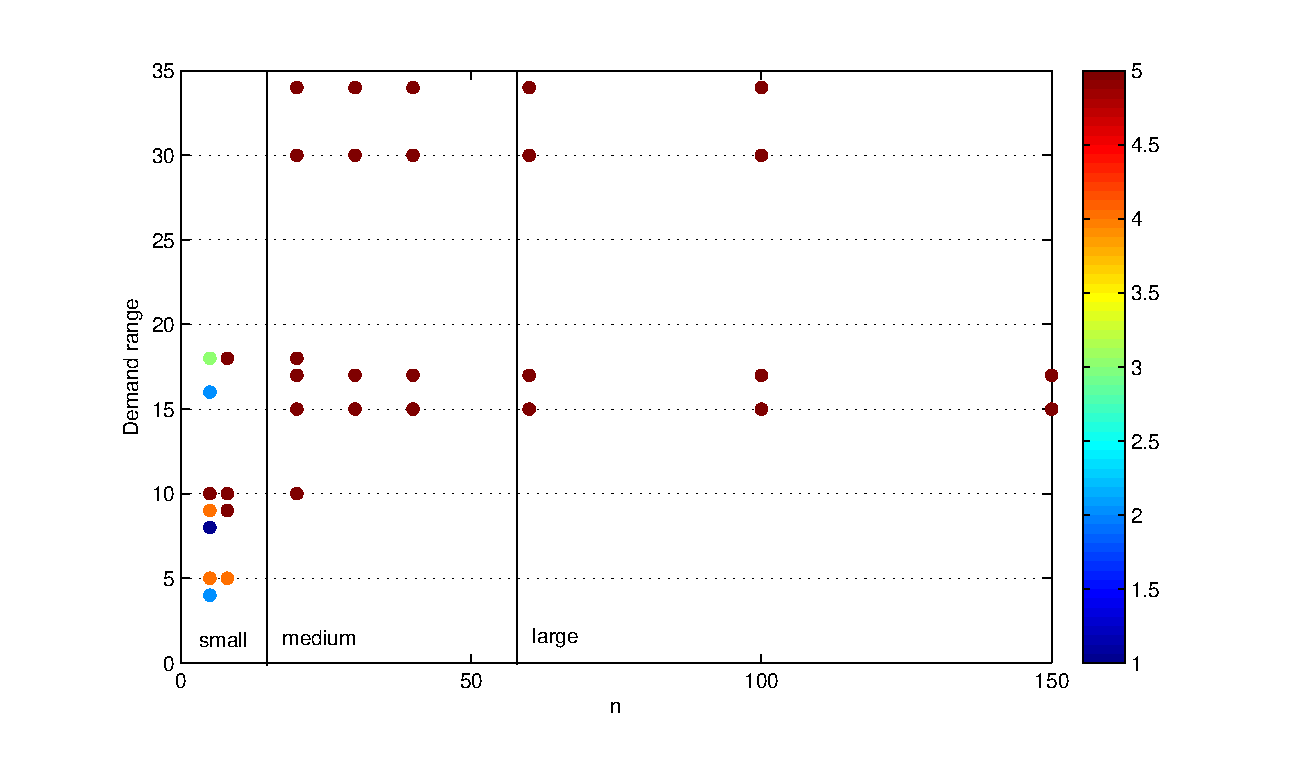
\includegraphics[width=0.6\textwidth]{Images/Chapter5/instances.eps}
  \end{center}
    \caption{Instance demands.}\label{fig:instances}
\end{figure}

instances with 



\begin{figure}[!htbp]
  \begin{center}
   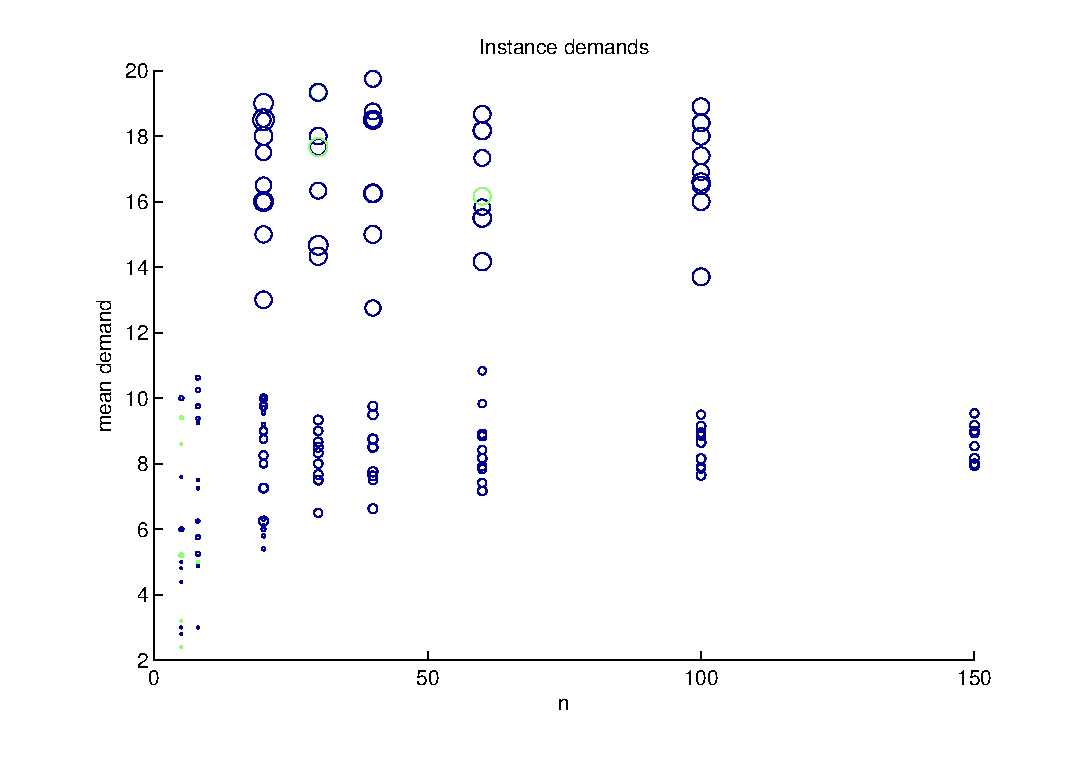
\includegraphics[width=0.8\textwidth]{Images/Chapter5/demands.eps}
  \end{center}
    \caption{Instance demands. Circles area represents the demand variance}\label{fig:demands}
\end{figure}

\section{Expected distance algorithm}\label{sec:test_expecteddistance}


In the figure \ref{fig:expected_distance3D_time}, we show the time consumed by algorithm $\Gamma$ \ref{algo:expecteddistance} to compute the expected distance for each instance. As expected, An higher value of $n$ and $Q$ increase the computational cost to compute expected distance. However, the figure \ref{fig:expected_distance3D_time} shows that the demands distribution affect the algorithm performance.

\begin{figure}[!htbp]
  \begin{center}
  \begin{subfigure}[h]{1\textwidth}
   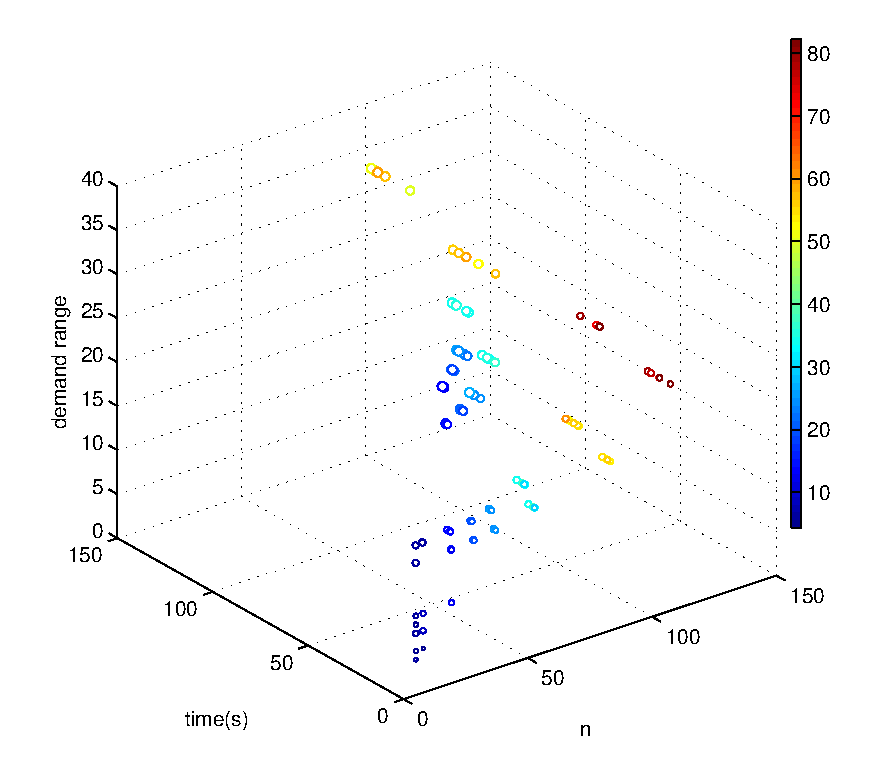
\includegraphics[width=0.7\textwidth]{Images/Chapter5/expected_distance3D.eps}
   \caption{Color shows expected distance to an arbitrary policy }\label{fig:expected_distance3D_time}
  \end{subfigure}
  \begin{subfigure}[h]{1\textwidth}
   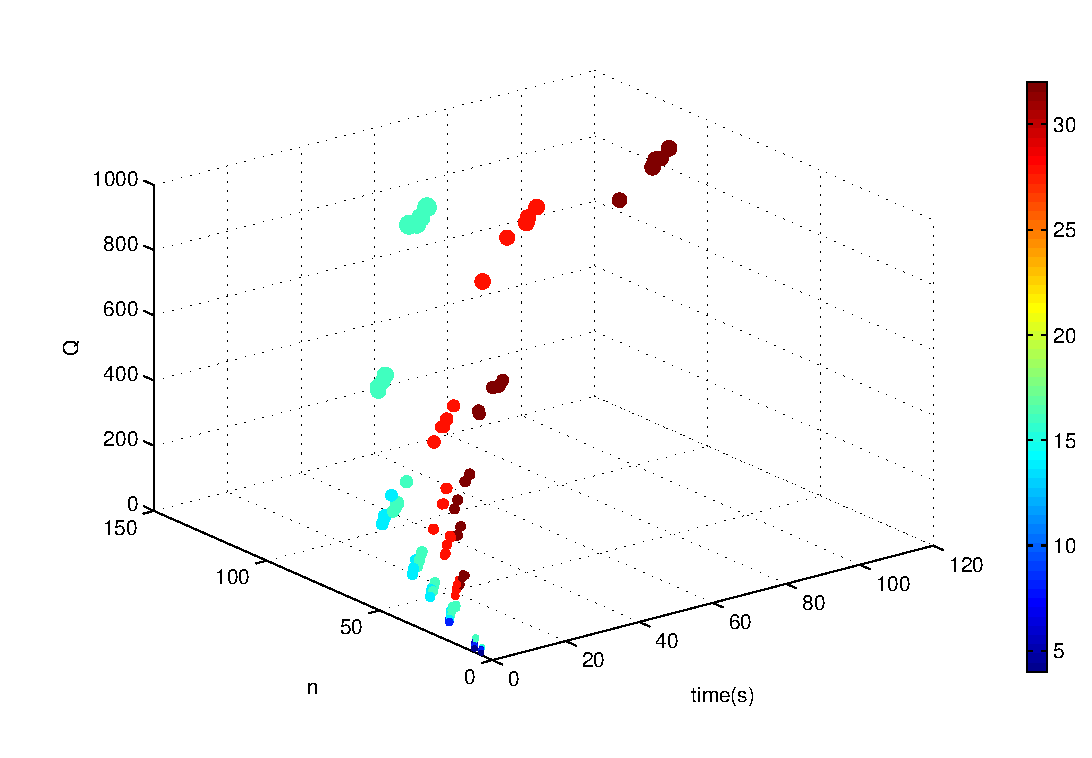
\includegraphics[width=0.7\textwidth]{Images/Chapter5/expected_distance3D_range.eps}
   \caption{color represents demand disribution}\label{fig:expected_distance3D_range_time}
  \end{subfigure}
   
  \end{center}
    \caption{Expected distance algorithm  $\Gamma$ performance}\label{fig:expected_distance3D}
\end{figure}

\clearpage

\section{Rollout algorithm}

In figure \ref{fig:ra_gamma_time_x2}, we put togeter the running time obtained by rollout algorithm and $\Gamma$ algorithm. Thus, we show experimentally the computational cost of rollout algorithm since this apply $O(n^2)$ times the $\Gamma$ algorithm.

\begin{figure}[!htbp]
  \begin{center}
   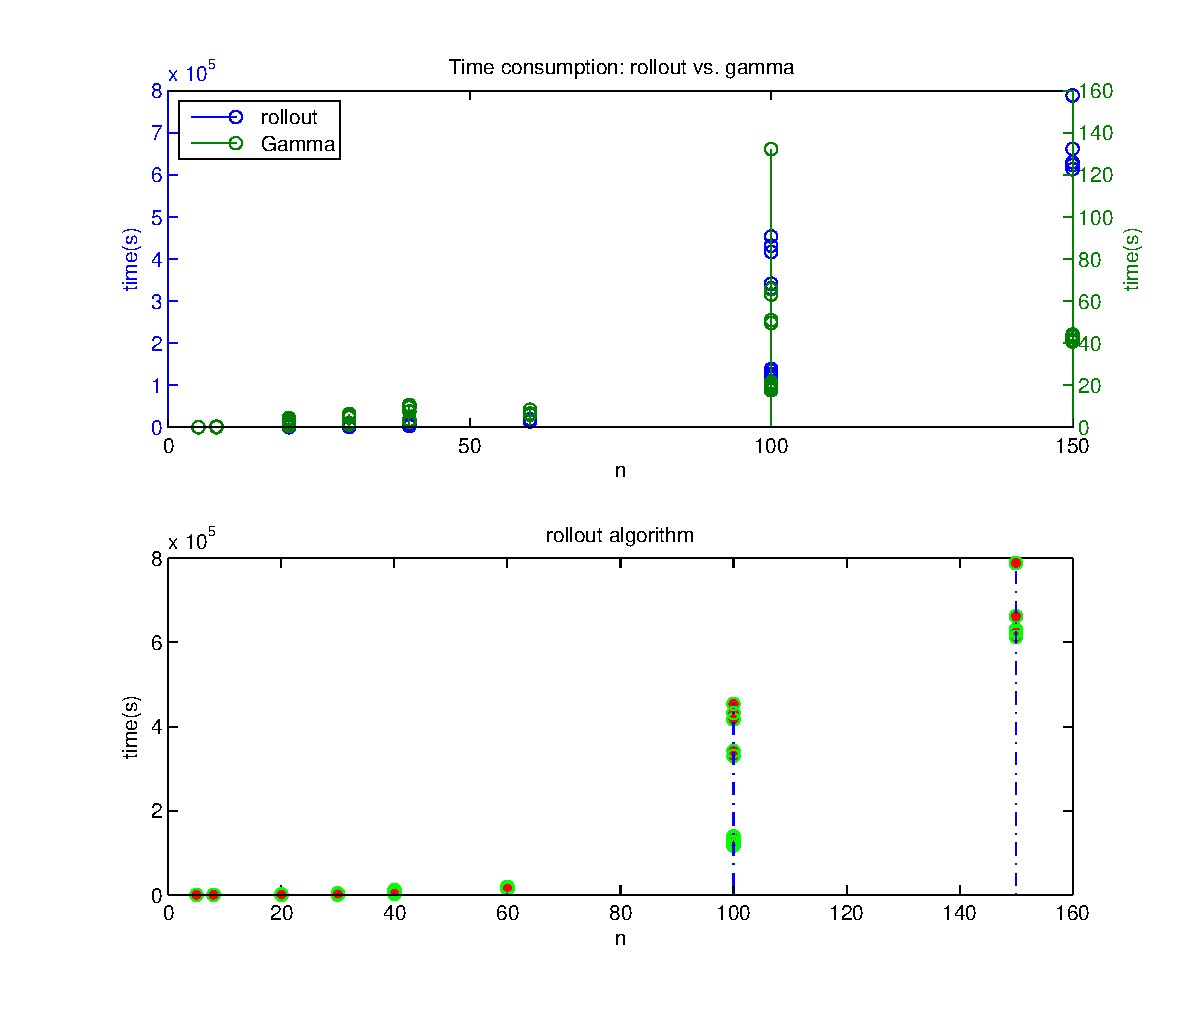
\includegraphics[width=0.9\textwidth]{Images/Chapter5/ra_gamma_time_x2.eps}
  \end{center}
    \caption{Performance rollout algorithm vs. $\Gamma$ algorithm}\label{fig:ra_gamma_time_x2}
\end{figure}


\begin{figure}[!htbp]
  \begin{center}
   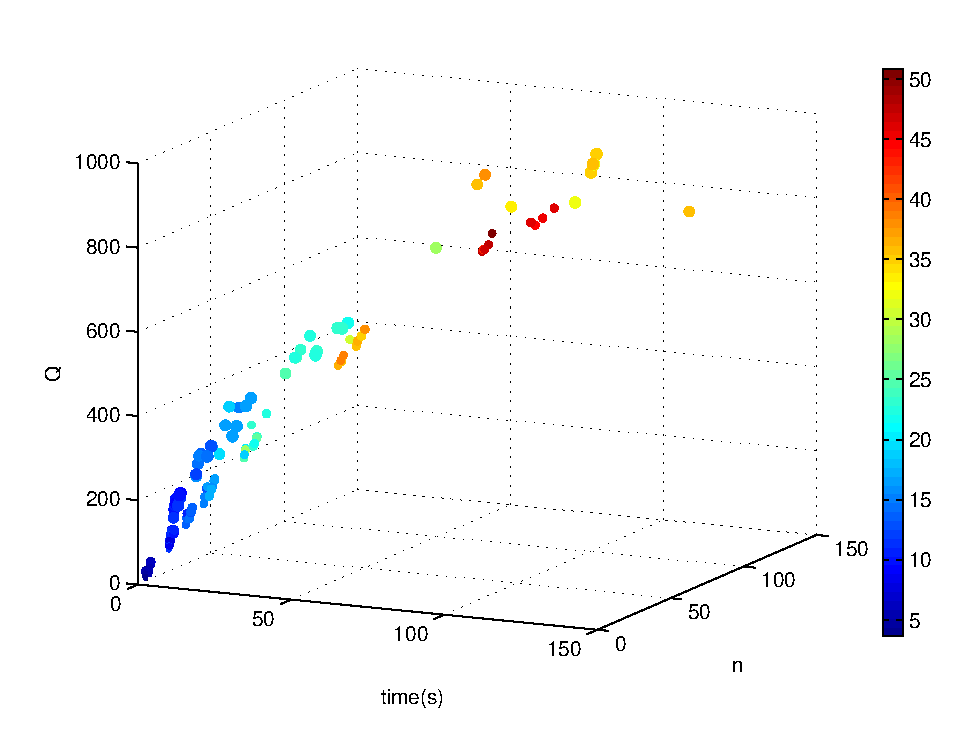
\includegraphics[width=0.9\textwidth]{Images/Chapter5/compare_expected_distance_ra.eps}
  \end{center}
    \caption{Performance rollout algorithm}\label{fig:compare_expected_distance_ra}
\end{figure}

\section{Evoulutionary approach}

We establish the values for the tunable parameters of genetic algorithm as a result of experimental obsevations. We selected a stratified sample of 10 instances and run basic genetic algorithm between 100 and 10 times the for each instance in the sample to compute a policy solution. Finally, we select the values for the parameters where the genetic algorithm otained the best average outcome.

Hence, we define the probability of mutation as $Prob_m = 0.04$ and the maximun counting of consecutive iterations without significative changing $\mathcal{m}$ as 10\% of the number of iterations and the stoping criterion to determine an significative as $\varepsilon = 1x10^{-3}$.

Others parameters were fixed to agree computational capability, such that  number of iterations $\kappa$ and size of population $\alpha$ since we recognize that a greater value for these increase the solutions explored. In concordace with the computational resoure available, we take $\kappa = 60$ and $\alpha = 0.5$

\subsection{Evolutionary algorithms performance}

In the figure \ref{fig:compare_expected_distance_ga}, we show the basic genetic algorithm outcomes for each problem instance.  For small instances the average expected value is 7.44 computed in an average time 1979 seconds (s), while medium and large size instances the average expected distance is 16.74 and 36.03 computed in an average time of 13033 s and 96357 s, respectively.


\begin{figure}[!htbp]
  \begin{center}
   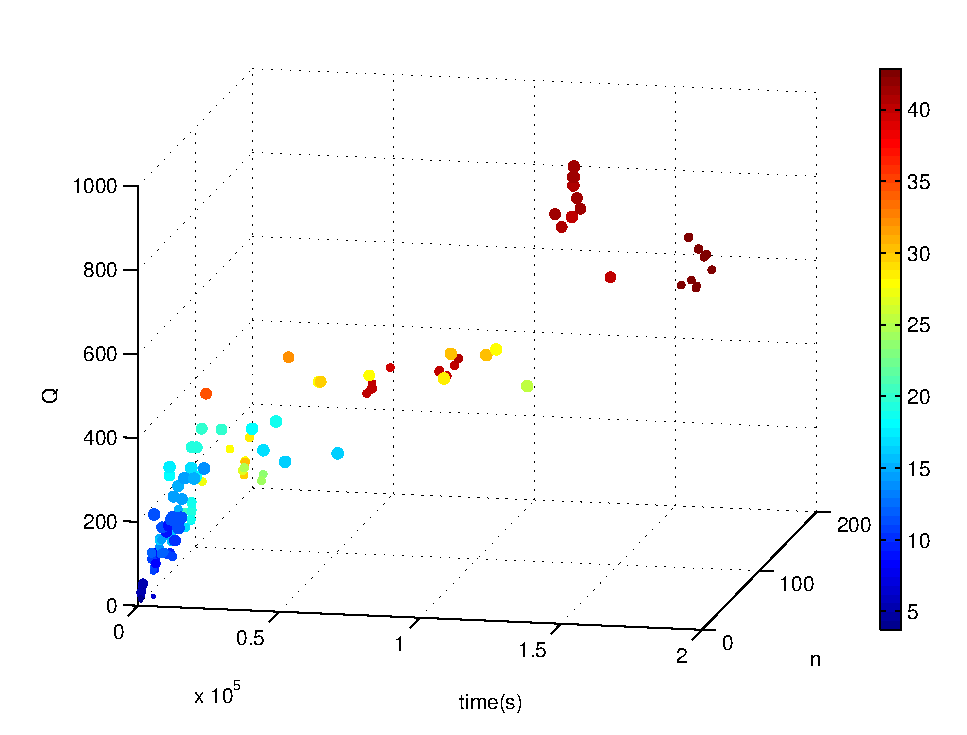
\includegraphics[width=0.7\textwidth]{Images/Chapter5/compare_expected_distance_ga.eps}
  \end{center}
    \caption{Performance basic genetic algorithm}\label{fig:compare_expected_distance_ga}
\end{figure}


Memetic algorithm finds better average results than basic genetic algorithm. Since that the hybrid genetic algorithm with rollout local search obtained an expected distance of 6.15, 10.99 and 16.67, to small, medium and large size instances, respectively. However these were computed longer, 
11441, 70460 and 123663 average seconds. Figure \ref{fig:compare_expected_distance_memetic} shows the expected distance computed for each instance in contrast with the running time expended.


\begin{figure}[!htbp]
  \begin{center}
   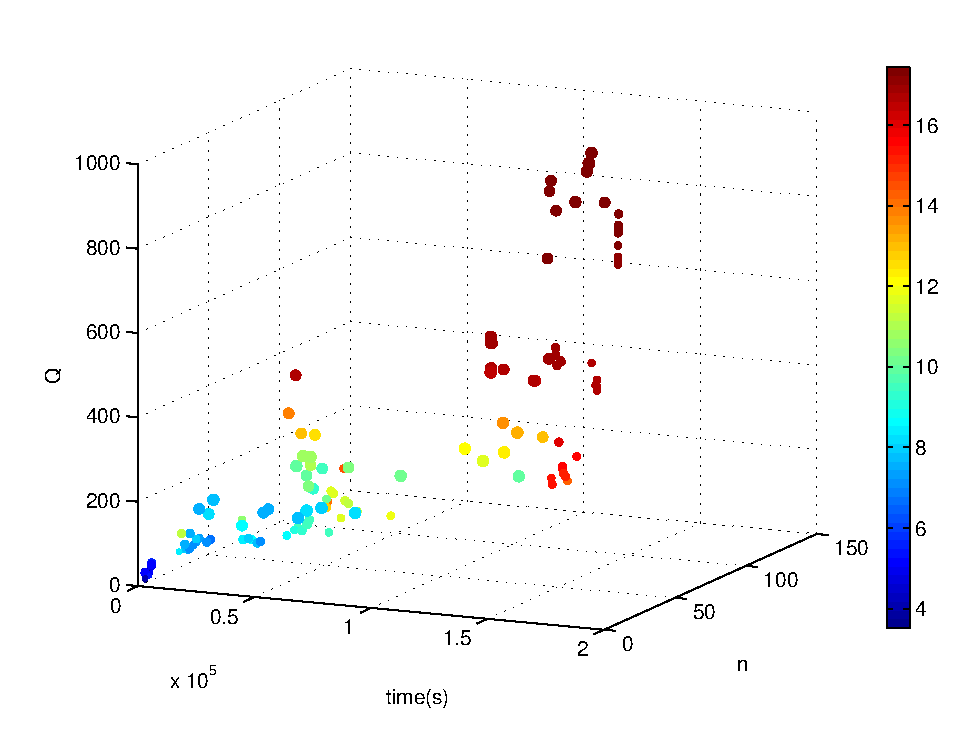
\includegraphics[width=0.7\textwidth]{Images/Chapter5/compare_expected_distance_memetic.eps}
  \end{center}
    \caption{Performance memetic algorithm}\label{fig:compare_expected_distance_memetic}
\end{figure}


In the behavior of the genetic algorithms, we observe that if local search is applied the evolutionary algorithm stops when the number of iterations is achived, rather than basic genetic algorithm where often complete the maximun counting of iterations without significative change. This can be observed in the figure \ref{fig:ga_basic_mvi_20r4_m} in comparison with the figure \ref{fig:memetic_mvi_20r4_m}.


\section{Comparative results}

We observe in the figure \ref{fig:comparative_results} as hybrid evolutionary algorithm beat both basic genetic algorithm as rollout algorithm. In fact, when instance size increase also grow the distance between the quality of solutions finded by memetic algorithm and the solutions computed by others.

\begin{figure}[!htbp]
  \begin{center}
   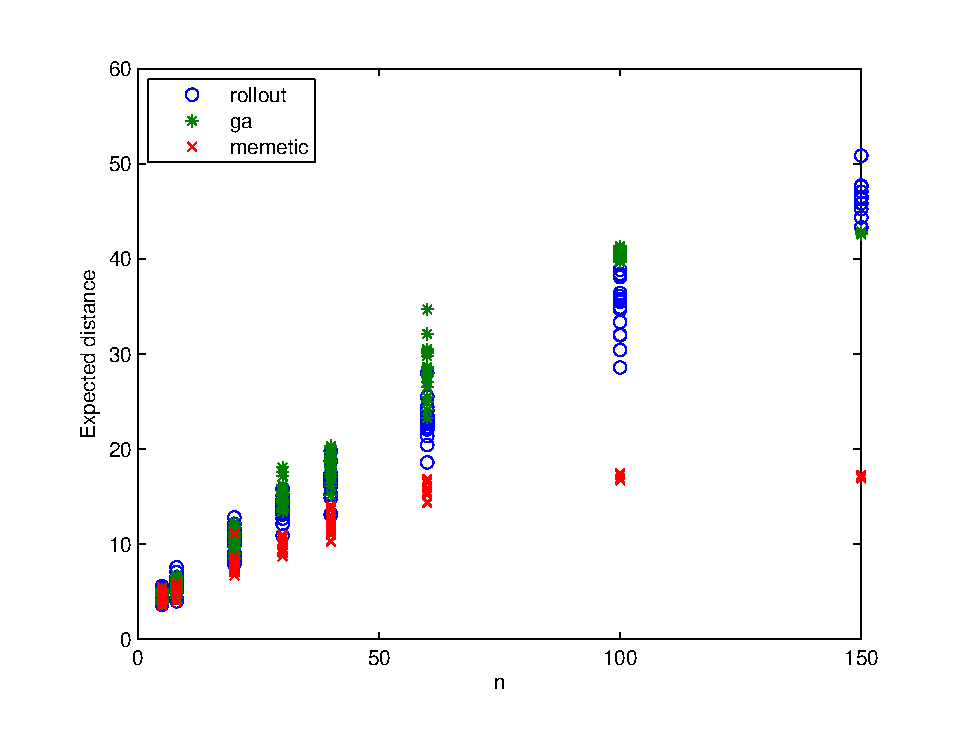
\includegraphics[width=0.8\textwidth]{Images/Chapter5/comparative_results.eps}
  \end{center}
    \caption{Expected distance computed by rollout algorithm (ra) , basic genetic algorithm (ga) and hybrid evolutionary algorithm (memetic)}\label{fig:comparative_results}
\end{figure}

Indeed, Not only memetic algorithm obtained better results than others algorithms implemented, also its outcomes have less variability, we observe this fact in the figure \ref{fig:comparative_results_box} where the hybrid evolutionary exhibit less variance in contrast with other techniques.

\begin{figure}[!htbp]
  \begin{center}
   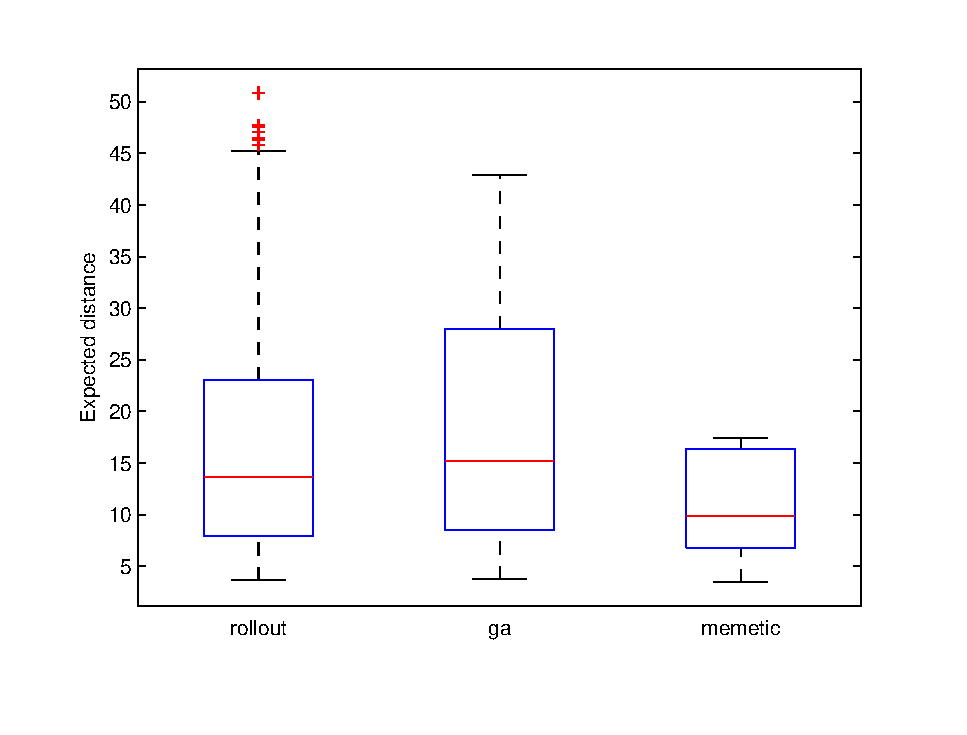
\includegraphics[width=0.9\textwidth]{Images/Chapter5/comparative_results_box.eps}
  \end{center}
    \caption{Boxplot for expected distance ra,ga,Memetic}\label{fig:comparative_results_box}
\end{figure}




In the figure \ref{fig:compare_times_evol}, we compare the execution time consumed by the evolutionary algorithms. In spite of that basic genetic algorithm often expend less time, the hybrid approach finds a solution employing less time for many large instances.

%subfigures:

\begin{figure}[!htbp]
  \begin{center}
   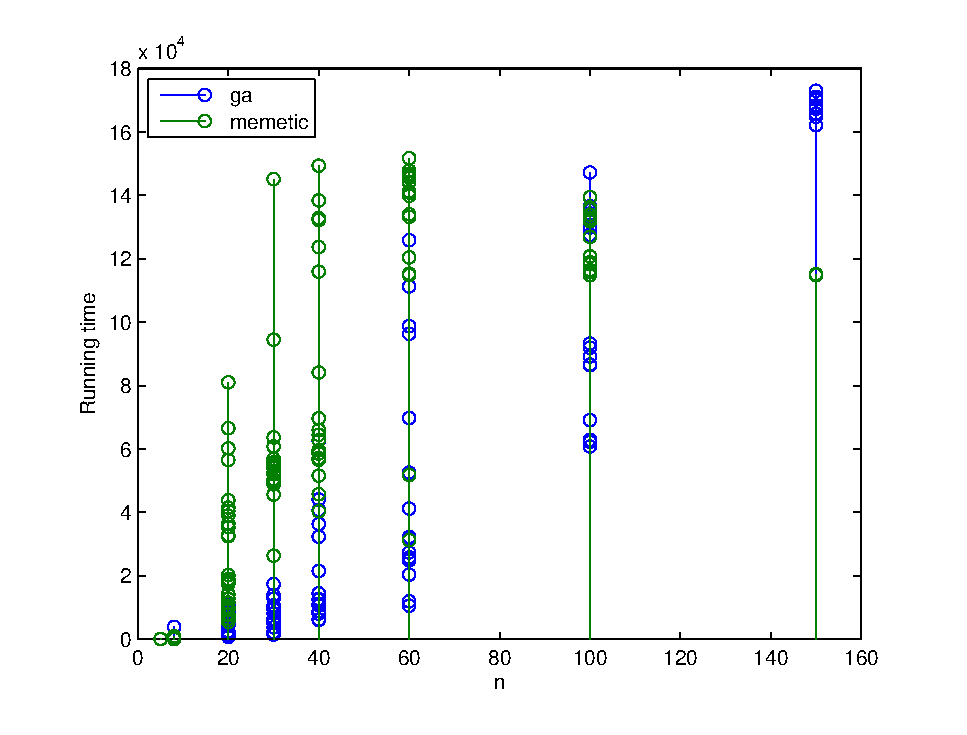
\includegraphics[width=0.8\textwidth]{Images/Chapter5/compare_times_evol.eps}
  \end{center}
    \caption{Time performance evolutionary algorithms}\label{fig:compare_times_evol}
\end{figure}

